\section{Parsing}

Dans cette section, nous décrivons la phase d'analyse syntaxique de notre interpréteur Mini-ML.

\subsection{Questions de compréhension}

\begin{enumerate}[label=\arabic*.]
    \item \label{question1}
          Nous avons commencé par réécrire une version simplifiée de notre grammaire dans Menhir, afin de générer le graphe LR(0) que nous souhaitions analyser.
          Pour cela, nous avons ajouté temporairement un token \texttt{T} dans le fichier \texttt{Tokens.mly}, ce qui nous a permis d’obtenir un automate représentatif de notre analyseur syntaxique.

          La grammaire utilisée est la suivante :

          \begin{lstlisting}[caption={Grammaire Menhir simplifiée}]
main:
| e = expr EOF { [(false, "result", e)] }

expr:
| FUN T ARROW e = expr   { Fun("x", e, Annotation.create $loc) }
| e1 = expr e2 = expr    { App(e1, e2, Annotation.create $loc) }
| T                      { Var("x", Annotation.create $loc) }
| L_PAR e = expr R_PAR   { e }
           \end{lstlisting}

          Ici, le non-terminal \texttt{main} est notre point d'entrée, et correspond à une expression suivie de \texttt{EOF}.
          L'utilisation du caractère \texttt{\textquotesingle} dans \texttt{expr\textquotesingle} a entraîné des complications.

          Après avoir généré le fichier \texttt{.dot} à l'aide de \texttt{Menhir}, nous avons utilisé la commande suivante pour obtenir une représentation graphique de l’automate sous forme d’image :

          \begin{lstlisting}[caption={Commande de génération de l'image}]
dot -Tpng Parser_sandbox.dot -o parser.png
          \end{lstlisting}

          Cette commande nous a permis d’obtenir le graphe LR(0) illustré ci-dessous, représentant les transitions entre les états de l’automate selon les règles définies dans notre grammaire :

          \begin{figure}[!ht]
              \centering
              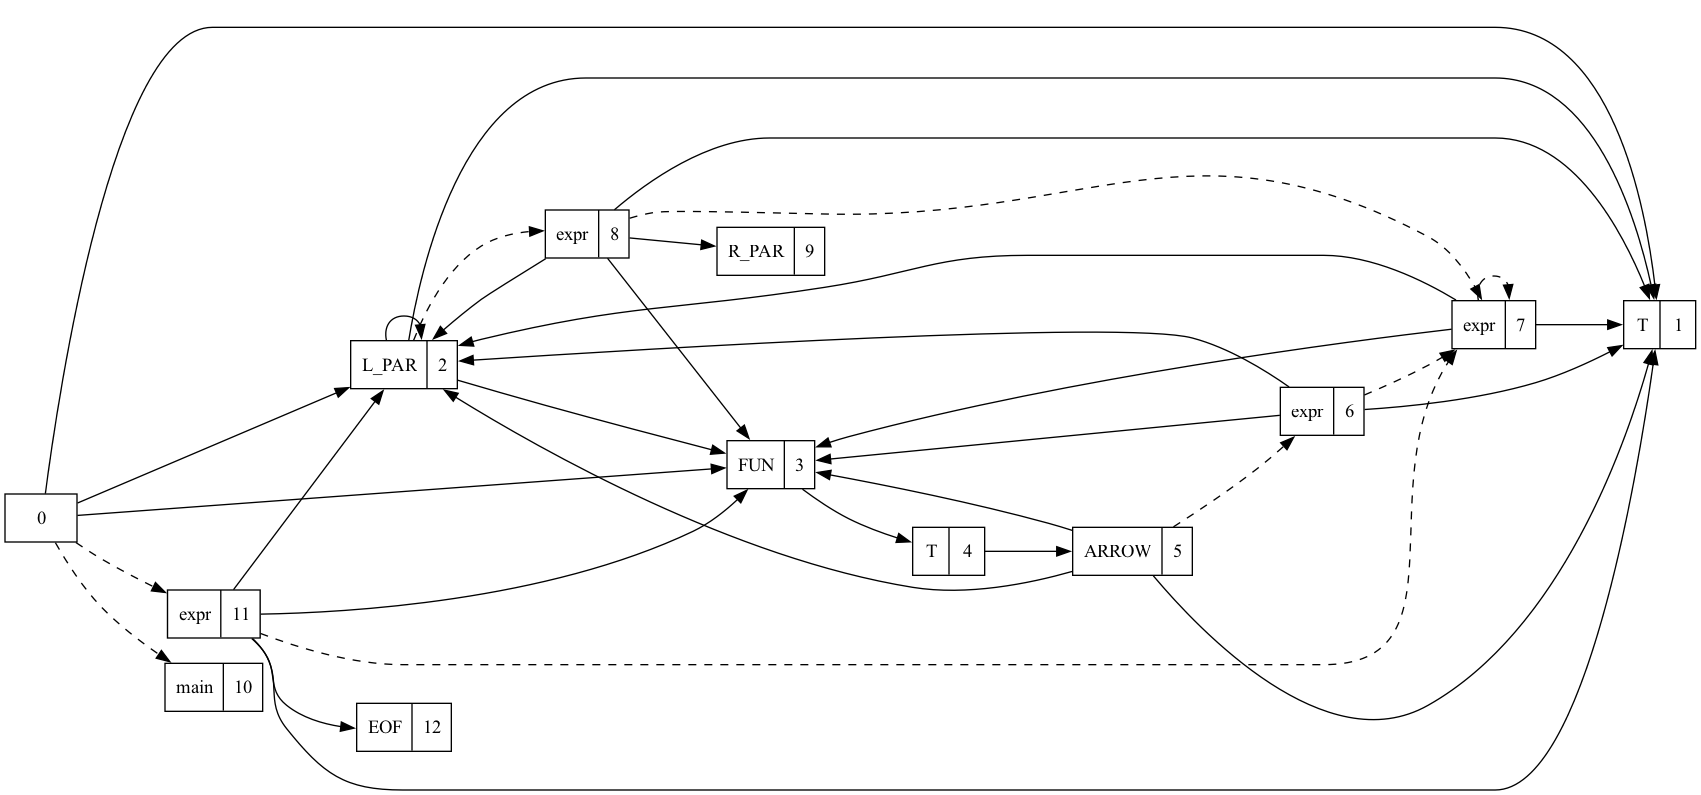
\includegraphics[width=1\textwidth]{images/L0Parser.png}
              \caption{Graphe généré à partir de la grammaire simplifiée}
              \label{fig:L0Parser}
          \end{figure}

          \newpage   % REMOVE THIS AFTER IDK %
          Nous n'étions pas satisfaits du graphe généré car il ne ressemblait pas aux graphes que nous avions vus dans le cours. Nous avons donc décidé de le créer manuellement et de le colorer.

          \begin{figure}[!ht]
              \centering
              \includegraphics[width=1\textwidth]{images/L0ParserAux.png}
              \caption{Graphe dessiné à partir de la grammaire simplifiée}
              \label{fig:L0ParserAux}
          \end{figure}

    \item \label{question2}
          Les conflits sur cet automate apparaissent dans les états 6 et 7.

          Dans l'état 7, un conflit de type shift/reduce survient car le parseur hesite entre réduire selon la règle \texttt{expr → expr expr} ou shifter sur les terminaux \texttt{T}, \texttt{L\_PAR} et \texttt{FUN}, étant donné que \texttt{expr} peut commencer par \texttt{T}.
          Dans l'état 6, un conflit shift/reduce existe entre la réduction selon la règle \texttt{expr → FUN T ARROW expr} et le shift sur les mêmes terminaux.
          Ces conflits s'expliquent par l'ambiguïté de la grammaire.

    \item \label{question3}
          Pour illustrer l’ambiguïté de cette grammaire, considérons la séquence de tokens suivante : \texttt{FUN T ARROW T T}.

          À première vue, on peut appliquer la règle \texttt{expr → FUN T ARROW expr}, ce qui conduit naturellement à une dérivation du type :
          \[
              \left( \texttt{FUN T ARROW T} \right) \ \texttt{T}
          \]

          Autrement dit, la première expression est interprétée comme une fonction prenant un argument et renvoyant une variable, puis appliquée à une seconde variable.

          Cependant, cette même séquence peut aussi être interprétée différemment en exploitant la règle \texttt{expr → expr expr}, qui autorise une application d’expressions. Ainsi, la dérivation suivante est également possible :

          \[
              \texttt{FUN T ARROW} \ \left( \texttt{T T} \right)
          \]

          Dans ce cas, l’expression entière est interprétée comme une fonction renvoyant l’application de deux variables.

          Cela reflète directement les conflits shift/reduce identifiés dans la question précedente de l’automate SLR, confirmant que la grammaire naturelle ne peut pas être analysée sans résoudre explicitement ces ambiguïtés.

    \item \label{question4}
          Le fichier \texttt{Parser\_calc.mly} définit la grammaire suivante :

          \begin{lstlisting}[caption={Grammaire du fichier \texttt{Parser\_calc.mly}}, label=lst:parser_calc, language=ocaml]
expr:
| e = simple_expr { e }
| FUN x = ID ARROW e = expr { Fun(x,e,Annotation.create $loc) }
| e1 = app_expr e2 = simple_expr { App(e1,e2,Annotation.create $loc) } 

simple_expr:
| i = INT { Cst_i(i,Annotation.create $loc) }
| f = built_in { Cst_func(f,Annotation.create $loc) }
| x = ID { Var(x,Annotation.create $loc) }
| L_PAR e = expr R_PAR { e }

app_expr:
| f = simple_expr { f }
| f = app_expr e = simple_expr { App(f,e,Annotation.create $loc)} 
          \end{lstlisting}

          Le parseur implementé renvoie exactement la dérivation:
          \[
              \texttt{FUN T ARROW} \ \left( \texttt{T T} \right)
          \]

          Il reconnait \texttt{FUN T ARROW} et entre dans la règle \texttt{expr -> FUN x = ID ARROW expr}. Pour \texttt{expr}, il voit \texttt{T T}, suite a app-expr, \texttt{app-expr -> (app-expr -> simple-expr T) simple-expr T}.

          Qui est exactement:
          \texttt{Fun("T", App(Var("T"), Var("T"), Annotation...), Annotation...)}.

    \item Si nous incluons toutes les fonctions built\_in dans l'analyseur et que nous voulons gérer correctement, nous devrons définir des priorités Menhir telles que \texttt{\%left, \%right et \%nonassoc}.

    \item La définition des non-terminaux permet de modéliser explicitement la structure syntaxique dans le cas d'applications fonctionnelles où l'association à gauche. Cette approche rend la grammaire plus lisible et plus facile à maintenir.

\end{enumerate}

\subsection{Syntaxe étendue}

Nous allons maintenant voir les modifications apportées au fichier \texttt{parser.mly}.

\subsubsection{Notation infixe des opérateurs binaire}

\subsection*{But}
Permettre à l'utilisateur d'écrire des expressions comme :
\begin{lstlisting}
2 + 1
x * 3 + 1
\end{lstlisting}

au lieu de devoir écrire la forme fonctionnelle explicite :

\begin{lstlisting}
(+) 1 2
\end{lstlisting}

\subsection*{État initial}

Dans la version initiale du parser, l'opérateur \texttt{+} était uniquement reconnu sous la forme fonctionnelle de type \texttt{(+ 1 2)} (c'est-à-dire avec des appels de fonction explicites). Cela signifiait que pour écrire des additions, les utilisateurs devaient utiliser une notation plus verbeuse et moins naturelle.

En revanche, l'opérateur \texttt{binop} pour les opérateurs arithmétiques et logiques était déjà défini, mais la grammaire ne reconnaissait pas encore la notation plus naturelle comme \texttt{1 + 2}.

\subsection*{Modification}
Afin d'améliorer la lisibilité et de rendre le langage plus proche d'une syntaxe standard (comme celle de OCaml), nous avons modifié la grammaire pour autoriser la notation infixée des opérateurs binaires comme \texttt{+}.

Nous avons utilisé la règle \texttt{binop} existante, mais en ajustant la manière dont l'opération est traitée dans la règle \texttt{expr}, de manière à reconnaître les opérateurs sous leur forme infixée.

\paragraph{Code modifié}
La règle \texttt{expr} a été modifiée pour permettre d'utiliser les opérateurs binaires de manière infixée, au lieu de nécessiter une notation fonctionnelle.

Par exemple pour ADD ici :
\begin{lstlisting}
| e1 = expr ADD e2 = expr {
    App(App(Cst_func(Add, Annotation.create $loc), e1, Annotation.create $loc), e2, Annotation.create $loc)
}
\end{lstlisting}

Puis nous avons modifié ceci \texttt{expr} pour utiliser la règle \texttt{binop} de manière générique :
\begin{lstlisting}
| e1 = expr op = binop e2 = expr {
    App(App(Cst_func(op, Annotation.create $loc), e1, Annotation.create $loc), e2, Annotation.create $loc)
}
\end{lstlisting}

\begin{itemize}
    \item Avant la modification, l'addition était seulement acceptée sous forme fonctionnelle explicite : \texttt{(+ 1 2)}.
    \item Après la modification, la notation infixée \texttt{1 + 2} est acceptée.
    \item La règle \texttt{binop} était déjà en place pour gérer les opérateurs comme \texttt{ADD}, \texttt{SUB}, etc. Nous avons utilisé cette règle pour reconnaître les opérateurs de manière plus naturelle, en l'intégrant dans \texttt{expr}.
\end{itemize}

\subsection*{Résultat}
Le parser accepte désormais les expressions suivantes :
\begin{lstlisting}
2 + 1
x * 3 + 1
\end{lstlisting}
et les transforme correctement dans l'AST, avec une structure homogène pour tous les opérateurs binaires.


\subsubsection{Ajout de la syntaxe \texttt{let f x y = e}}
\subsection*{But}
Permettre une définition plus naturelle des fonctions multi-arguments sans passer par des \texttt{fun} imbriqués.

\subsection*{État initial}
Dans la version originale du parser, la règle \texttt{req} reconnaissait uniquement des définitions de la forme :
\begin{lstlisting}
LET name = ID EQ expr
LET REC name = ID EQ expr
\end{lstlisting}

Autrement dit, une déclaration était limitée à :
- Un nom de fonction ou variable
- Le mot-clé \texttt{let} ou \texttt{let rec}
- Une expression affectée à ce nom (souvent un \texttt{fun} explicite dans le cas d’une fonction)

Cela forçait l’utilisateur à écrire des \texttt{fun} imbriqués manuellement.

\subsection*{Modification}
Pour autoriser des définitions avec plusieurs arguments de manière plus lisible, nous avons :
\begin{enumerate}
    \item Créé une règle auxiliaire \texttt{many\_args} qui reconnaît une suite d’identifiants représentant les arguments formels.
    \item Modifié la règle \texttt{req} pour inclure ces arguments après le nom de la fonction.
    \item Utilisé \texttt{List.fold\_right} pour convertir les arguments en une série de fonctions.
\end{enumerate}

Ajout d'une règle auxiliaire \texttt{many\_args} qui permet de reconnaître une séquence d'identifiants représentant les arguments de la fonction :

\begin{lstlisting}
many_args:
| { [] }
| id = ID args = many_args { id :: args }
\end{lstlisting}

Modification de la règle \texttt{req} :

\begin{lstlisting}
req:
| LET name = ID args = many_args EQ e = expr {
    let fun_expr = List.fold_right (fun arg acc -> Fun(arg, acc, Annotation.create $loc)) args e in
    (false, name, fun_expr)
}
| LET REC name = ID args = many_args EQ e = expr {
    let fun_expr = List.fold_right (fun arg acc -> Fun(arg, acc, Annotation.create $loc)) args e in
    (true, name, fun_expr)
}
\end{lstlisting}

\subsection*{Résultat}
Syntaxe acceptée :
\begin{lstlisting}
let add x y = x + y
\end{lstlisting}

Donc :
\begin{itemize}
    \item La fonction \texttt{List.fold\_right} construit l'AST de type \texttt{Fun} en partant du dernier argument.
    \item Chaque argument devient un nœud \texttt{Fun(arg, ...)} imbriqué autour du corps \texttt{e}.
    \item Ainsi, \texttt{let f x y = e} devient \texttt{Let("f", Fun("x", Fun("y", e)))}.
\end{itemize}

\subsubsection{Ajout du \texttt{-} unaire (moins)}

\subsection*{But}
Permettre à l'utilisateur d'écrire des expressions comme :
\begin{lstlisting}
-4
-(x + 1)
\end{lstlisting}
au lieu d’utiliser la version fonctionnelle explicite :
\begin{lstlisting}
neg 4
\end{lstlisting}
\subsection*{État initial}
Avant la modification, le parser ne reconnaissait que l'opérateur unaire \texttt{neg}, défini comme une constante fonctionnelle dans l’AST :
\begin{lstlisting}
| NEG { UMin }
\end{lstlisting}
Son usage nécessitait d'écrire des expressions comme \texttt{neg x}, ce qui est moins naturel que d'utiliser \texttt{-x}.

De plus, dans la grammaire, le token \texttt{SUB} était uniquement associé à l’opérateur binaire de soustraction :
\begin{lstlisting}
e1 = expr SUB e2 = expr { ... }
\end{lstlisting}
Ce qui provoquait un conflit de priorité si on voulait le réutiliser pour l'usage unaire.

\subsection*{Modification}
Nous avons introduit la prise en charge explicite de l'opérateur unaire \texttt{-} en modifiant la grammaire à deux niveaux :
\begin{enumerate}
    \item Ajout d’une directive de précédence \texttt{\%right NEG} en haut du fichier, pour qu’il soit correctement priorisé par rapport aux opérateurs binaires.
    \item Ajout d’une règle dans \texttt{expr} pour reconnaître l’usage de \texttt{-} en position préfixe (unaire).
\end{enumerate}

\paragraph{Code modifié}
Ajout dans les règles d'expressions :
\begin{lstlisting}
| SUB e = expr %prec NEG {
    App(Cst_func(UMin, Annotation.create $loc), e, Annotation.create $loc)
}
\end{lstlisting}

\subsection*{Résultat}
Le parser comprend désormais les expressions suivantes :
\begin{lstlisting}
-4
-x + 2
\end{lstlisting}

\subsubsection{Support des listes avec \texttt{[a; b; c]} et \texttt{[]}}

\subsection*{But}
Permettre à l'utilisateur de créer des listes de manière intuitive, comme en OCaml :
\begin{lstlisting}
[1; 2; 3]
[]
\end{lstlisting}

\subsection*{État initial}
Dans la version de base, les listes n’étaient pas prises en charge ou nécessitaient une construction explicite avec l’opérateur \texttt{::}.

\subsection*{Modification}
Nous avons ajouté une règle dédiée dans \texttt{simple\_expr} pour reconnaître les crochets \texttt{[...]} et les expressions séparées par \texttt{;}.

Dans \texttt{simple\_expr} :
\begin{lstlisting}
| L_SQ R_SQ { Nil(Annotation.create $loc) } 
| L_SQ l = separated_nonempty_list(SEMICOLON, simple_expr) R_SQ {
    let loc = Annotation.create $loc in
    List.fold_right (fun elt acc -> 
        App(App(Cst_func(Cat, loc), elt, loc), acc, loc)) l (Nil loc)
}
\end{lstlisting}

\subsection*{Résultat}
Le parser peut maintenant transformer des expressions comme :
\begin{lstlisting}
[1; 2; 3]
\end{lstlisting}
en un AST équivalent à :
\begin{lstlisting}
1 :: 2 :: 3 :: []
\end{lstlisting}
avec l'opérateur \texttt{Cat} utilisé récursivement via \texttt{fold\_right}.

\subsubsection{Support de la notation \texttt{f x y}}

\subsection*{But}
Permettre les appels de fonctions comme :
\begin{lstlisting}
f x y
\end{lstlisting}

\subsection*{Modification}
Nous avons introduit une règle \texttt{app\_expr} récursive à gauche, permettant de construire des appels multiples de la forme \texttt{f x y} comme des applications successives imbriquées.

\begin{lstlisting}
app_expr:
| f = simple_expr { f }
| f = app_expr e = simple_expr {
    App(f, e, Annotation.create $loc)
}
\end{lstlisting}

\subsection*{Résultat}
Un appel comme :
\begin{lstlisting}
f x y
\end{lstlisting}
est transformé dans l’AST en :
\begin{lstlisting}
App(App(Var("f"), Var("x")), Var("y"))
\end{lstlisting}
et ce, de manière récursive pour autant d'arguments que souhaité.